\graphicspath{{../images/intro/}}
\chapter{Постановка задачи и обзор существующих методов}
\section{Немного о белках. Основные определения}
% - что такое белки
% - из чего состоят
% - что такое поверхность белка
% - информация о вторичной структуре 
%(мб сказать что такое вторичная структура белка?  вынести во введение или первую главу)
Зачастую являясь результатом несинонимичной замены одного нуклеотида, точечная мутация одной аминокислоты может приводить к масштабным последствиям: так, например,
\subsection{Белки как основа живой материи}
\textbf{Первичная структура} белка задается последовательностью (\textbf{цепочкой}) аминокислот:

\resizebox{0.9\textwidth}{!}{
%\input{aa3_5.tex}
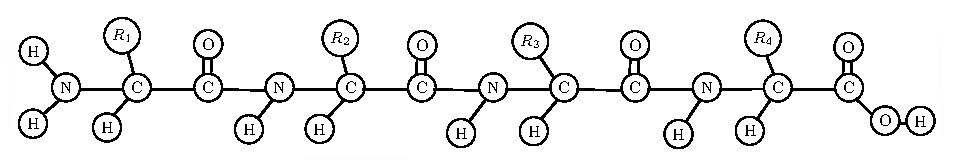
\includegraphics{aa3_1.eps}
}

\textbf{Вторичная структура} задается укладкой цепочки аминокислот в пространственные структуры, \textbf{третичная структура} - расположением этих структур в пространстве в случае, когда белок содержит только одну цепь.

Когда белок состоит из нескольких цепей, говорят о его \textbf{четвертичной структуре}.

\subsection{Белки и энергия}
С точки зрения химии, разным видам структуры соответствуют разные виды химических связей и электростатических взаимодействий.

Когда мы рассматриваем несколько цепочек в составе одного белка или несколько белков, образующих комплекс, мы говорим о \textbf{белок-белковом взаимодействии}.

\textbf{Интерфейс} такого взаимодействия -- это участки \textbf{поверхности} белков, непосредственно контактирующие между собой.

Свободная энергия связи, обозначаемая \ddG, определена как разность $\vartriangle\!G_{mut} - \vartriangle\!G_{wt}$ , где $\vartriangle\!G_{wt}$ и $\vartriangle\!G_{mut}$ -- изменения свободной энергии Гиббса для немодифицированного белка (как еще перевести wild-type?? чтоб не в лоб) и его подвергнутой точечному мутагенезу версии (alanine-mutated
protein).
\newpage
\subsection{Поверхность белка как его энергетический фронт}
\subsection{Белок-белковое взаимодействие}
Рассмотрим белок, имеющий четвертичную структуру.

\textbf{Вопрос}: можно ли изменить что-то в его структуре, чтобы образующие его цепочки были лучше сцеплены между собой?

Пусть есть комплекс из двух белков (например, имунноглобулин и эпитоп).

\textbf{Вопрос 1}: можно ли изменить что-то в его структуре, чтобы усилить связь между компонентами комплекса?

\textbf{Вопрос 2}: насколько специфична одна из компонент комплекса?  Можно ли подобрать один из белков так, чтобы комплекс был более устойчивым? Насколько заменяема каждая из компонент?

Ответить нам поможет \textbf{аланиновое сканирование} (аланиновый мутагенез).
\newpage
\section{Аланиновое сканирование}
Аланиновое сканирование (ала-скан)~\cite{alascan2001} - метод для определения аминокислот в составе белка, играющих важную роль в сохранении его функций, стабильности или формы.

Первоначальная идея метода очень проста: заменить одну из аминокислот в цепочке на любую другую и посмотреть, повлияет ли такое точечное изменение (точечный мутагенез) на энергию комплекса, приведет ли это к усилению или ослаблению взаимодействия между цепочками белков. 
\begin{center}
\resizebox{0.4\textheight}{!}{
\ttfamily
\footnotesize
\aapicture
}
\end{center}

Но как выбирать аминокислоту, на которую проводить замену? Всегда ли стоит перебирать все аминокислоты в одной и той же позиции в цепочке?

 Экспериментально было показано~\cite{alascan2001}, что достаточно заменить аминокислоту на аланин, чтобы понять, является ли она энергетически значимой при оценке взаимодействия цепочек, или нет. А затем, если изменение энергии комплекса \ddG  оказывается существенным, перебрать все оставшиеся аминокислоты в данной позиции и определить, какая замена является экстремальной.

\begin{wrapfigure}{RT}{0.3\textwidth}
\resizebox{0.3\textwidth}{!}{
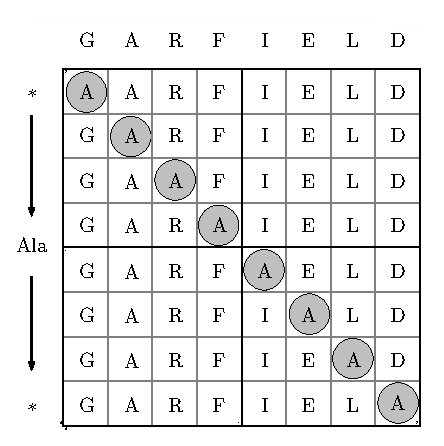
\includegraphics{ala_scan.eps}
}
\end{wrapfigure}
\newpage
\subsection{Аланиновое сканирование in vitro/in vivo}
Первоначально аланиновое сканирование появилось как лабораторный, химический метод (in vitro/in vivo), с вытекающими отсюда недостатками:
\begin{itemize}
\item Большое пространство поиска: для того, чтобы определить энергетически значимые аминокислоты, требовалось проверить все.
\item Сложность синтеза библиотек: необходим индивидуальный подход, сложность с разделением образцов с мутациями, сложность получения образцов с точечной мутацией в нужной позиции.
\item как следствие, высокая стоимость.
\end{itemize}

Впоследствии появились базы данных с результатами аланинового сканирования ~\cite{asedb2001, bid2003}, но они фрагментированы, не всегда полны, разнородны. Кроме того, данных в них не так много - в силу приведенных выше недостатков проведения точечного мутагенеза в лаборатории.

Например, если Protein Data Bank содержит информацию о большом количестве структур, с примерно одним и тем же форматом данных, то asedb представляет собой базу данных mysql и содержит информацию о 101 структуре, а bid доступен в виде набора wiki-страниц с информацией о конкретных белках или парах взаимодействующих цепочек.
%уточнить цифру
 \newpage
\subsection{Аланиновое сканирование in silico: решаемые задачи и границы применимости}
\todo{написать про метод, протоколы, используемые функции, что такое дельта-дельта G}

\todo{сказать, что в данной работе используется протокол из rosetta (мб привести картинку про реальную ddG и in silico функцию изменения энергии), сцепленность цепочек оценивается в смысле изменения энергии, применяемый в протоколе метод монте-карло лежит за пределами работы (кроме того, является относительно хорошо изученным, в ходе работы никакие модификации в сам метод или функцию оценки ddG не вносились), поэтому не приводится. }

\newpage
\section{Стандартные методы выбора аминокислот для аланинового сканирования in silico}

Как правило, при компьютерном моделировании аланинового сканирования применяют предварительную фильтрацию аминокислот, после которой проводится сканирование. Для фильтрации используются два основных метода~\cite{hotspots2012rev}:
\begin{itemize}
\item отсечка по расстоянию ~\cite{kortemme2004}: мутации подвергаются только те аминокислоты, которые расположены вблизи области взаимодействия пары белков;

\item выбор по гомологии: аминокислоты выбираются исходя из имеющихся экспериментальных результатов аланинового сканирования, проводившихся на близких (в эволюционном смысле) последовательностях.
\end{itemize}

Оценим эффективость этих подходов.

\subsection{Использование отсечки по расстоянию}

\begin{itemize}
\item Аланиновому сканированию подвергаются аминокислоты цепочки, образующей комплекс совместно с другой цепочкой, содержащие атомы, удаленные от каких-либо атомов цепочки, также участвующей в образовании комплекса, на расстояние, не превышающей некоторой фиксированной величины

\item В качестве порогового значения расстояния используются, например, величины 4, 5, 8 \AA{}

\item в Rosetta Alascan Protocol~\cite{kortemme2004} используется усложнение: дополнительно рассматриваются аминокислоты, $\beta$-углерод которых после формирования комплекса в шаре определенного фиксированного радиуса содержит существенно больше атомов $\beta$-углерода, чем содержал до этого.
\end{itemize}
\newpage
Эксперимент
\begin{itemize}
\item Рассмотрим базу данных с информацией о результатах эспериментов по аланиновому сканированию белков ASEdb~\cite{asedb2001}.
\item Найдем объекты с корректными ссылками на записи в Protein Data Bank ~\cite{rcsb}.
\item Среди всех таких объектов, найдем те, в которых есть аминокислоты, мутация которых приводит к существенному изменению свободной энергии комплекса ($\geq 1$ ккал/моль)
\item Посмотрим, всегда ли они удалены от интерфейса в пределах стандартно используемой отсечки (в качестве примера возьмем расстояние, не превышающее 8 \AA{}).
\end{itemize}

\resizebox{0.8\textwidth}{!}{
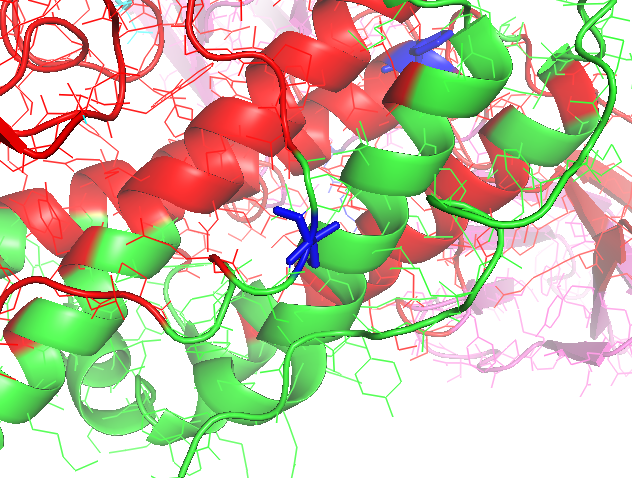
\includegraphics{image7.png}
}

\newpage
\subsection{Поиск по гомологии}
Для эффективного поиска по гомологии необходимо иметь базу близких (ортологичных) структур, точную и содержащую всю информацию по результатам аланинового сканирования.

Метод должен учитывать как данные о последовательности аминокислот в белках, так и каким-либо образом эксплуатировать пространственную структуру. В качестве примеров методов, учитывающих и то, и другое, можно привести ~\cite{hhm_svm}.

Проводятся попытки классификации участков, 
%здесь можно ссылку на диссертацию студентки Фришмана
